\section{Background}

\subsection{Radiation experiments}
Radiation experiments made in specialized facilities, where a neutron-radiation accelerator may lie, are used to evaluate the reliability of computer systems such as \textbf{FPGAs}, \textbf{CPUs}, and \textbf{ASICS} in an environment of high radiation. The most common use of the data gained from such experiments is to strengthen systems to survive in space. 

For a radiation experiment to succeed, some prerequisites are required. The most important of them is that people mustn't enter the room where charged particles are present. To accomplish this, specialized software must be made to autonomously control the systems under test inside the accelerator's room. Continuing in the current chapter, we will introduce a framework that is used to ensure both the safety of people and the integrity of the data gained in an experiment in which high radiation is present.

\subsection{Symphony}
As stated in previous chapters, Symphony constitutes a framework leveraged for conducting radiation experiments. To accomplish this, Symphony lets users customize the necessities required for an experiment. The framework provides the user with an API to instruct Symphony to handle certain crucial situations.


The Sympohy's API provides the following basic functionalities for radiation experiments:
\begin{itemize}
  \item A way to define the benchmarks to execute during the experiment
  \item A way to handle crucial situations, such as kernel panic, crashes, and more (as depicted \autoref{tab:symphony_handle}).
  \item Give the user the freedom to choose what to do in the most common situations expected in such an experiment (through some callbacks, which will be covered later). 
  \item Saves the results in easy process JSON files.
\end{itemize}

\begin{table}[h!]
\begin{center}
\begin{tabular}{ |c|c|c| } 
\hline
Situation & Handle \\
\hline
Kernel Panic & Restart \\ 
PL Crash & Restart \\  
SDCs  & LOG \\
Netowrk Error & LOG \\
System Error (recovered) & LOG \\

\hline
\end{tabular}
\caption{Crusial situations handled by Symphony}
\label{tab:symphony_handle}
\end{center}
\end{table}

\subsubsection{Architecture}
Symphony's architecture uses the Client-Server network model. As the model suggests, it uses the network infrastructure to establish a connection between two systems, one located inside the radiation room, called Device Under Test (DUT), and the other that controls the DUT device from outside, called Host. The Host is responsible for the client-side operations, while the DUT is responsible for the server side.

The architecture of Symphony can be depicted in \autoref{fig:symphony_architecture_ilustrate}. As illustrated in \autoref{fig:symphony_architecture_ilustrate}, the Host and \textbf{DUT} are connected using a gateway router. Another detail spotted in the figure is an entity called "LOGIC" and "CALLBACK" both clarified later in this sentence.  Logic constitutes hardware responsible for performing a hard reset on the DUT system. Callback, if we overuse the original terminology, it can be called a "driver". This callback instructs Symphony to perform a hard reset, when necessary, using the so-called "LOGIC" hardware in between. 

\begin{figure}[h]
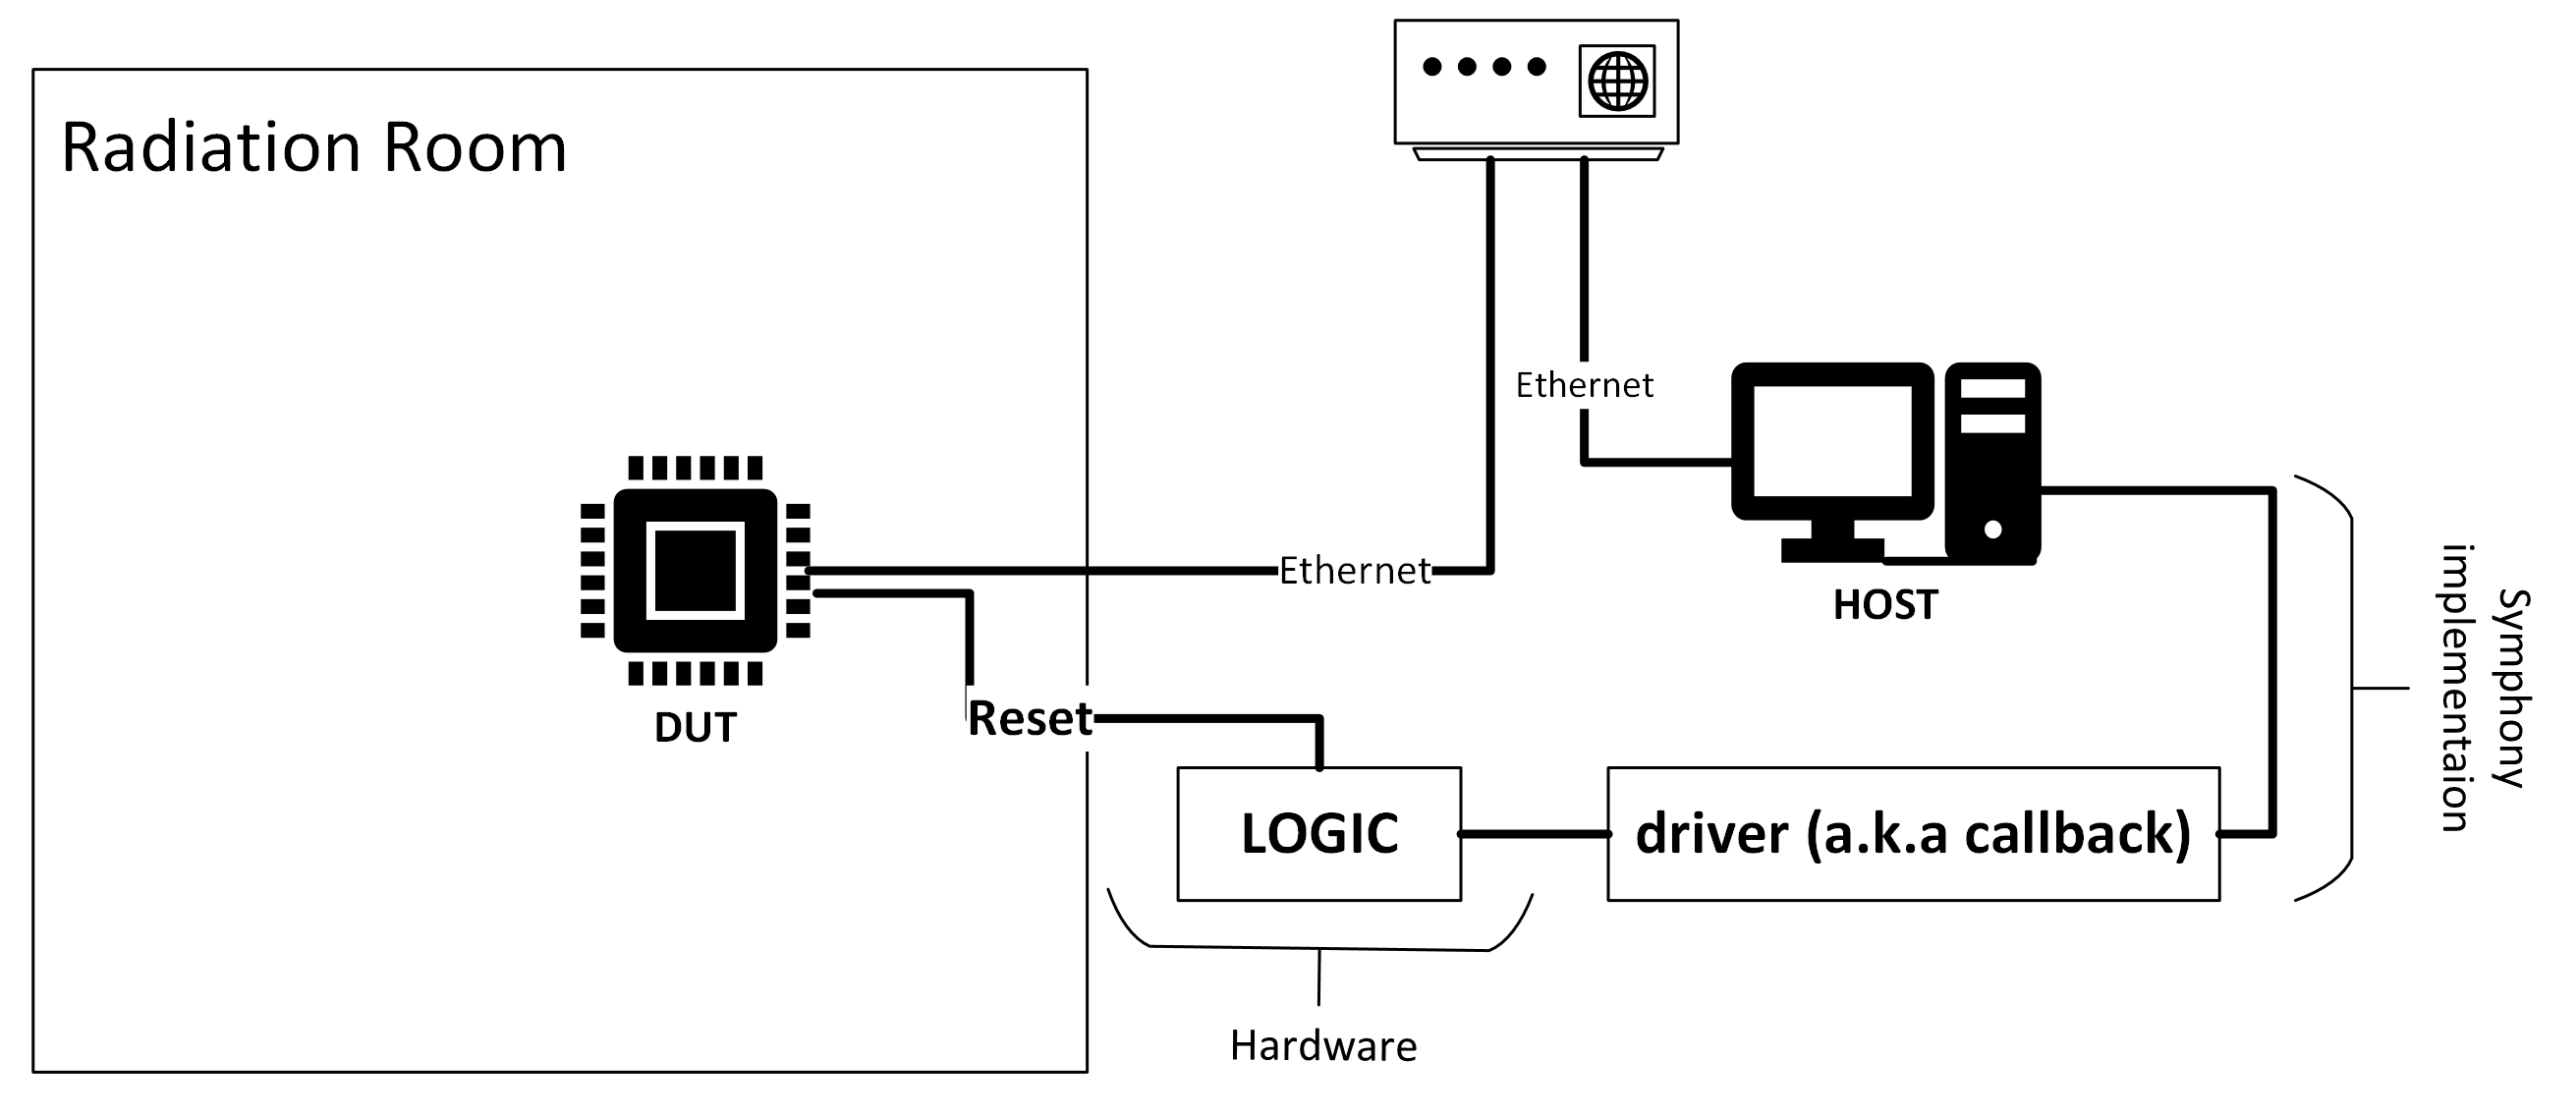
\includegraphics[width=\textwidth]{images/symphony.png}
\centering
\caption{Symphony's Architecture}
\label{fig:symphony_architecture_ilustrate}
\end{figure}

The driver (a.k.a. callback) is user-defined and varies between implementations. Section \ref{sec:user_defined_callbacks} describes how the callback is defined and how to implement such a routine.

\subsubsection{Device Under Test}
As depicted in \autoref{fig:result_message_dut}, the DUT is located inside the experiment room. This device is responsible for executing any command requested from the Host. Another task is to send back, through the network infrastructure, the results of the executed commands. The message that contains the result is in a specified dictionary format, shown in \autoref{fig:result_message_dut}.

\begin{figure}[h]
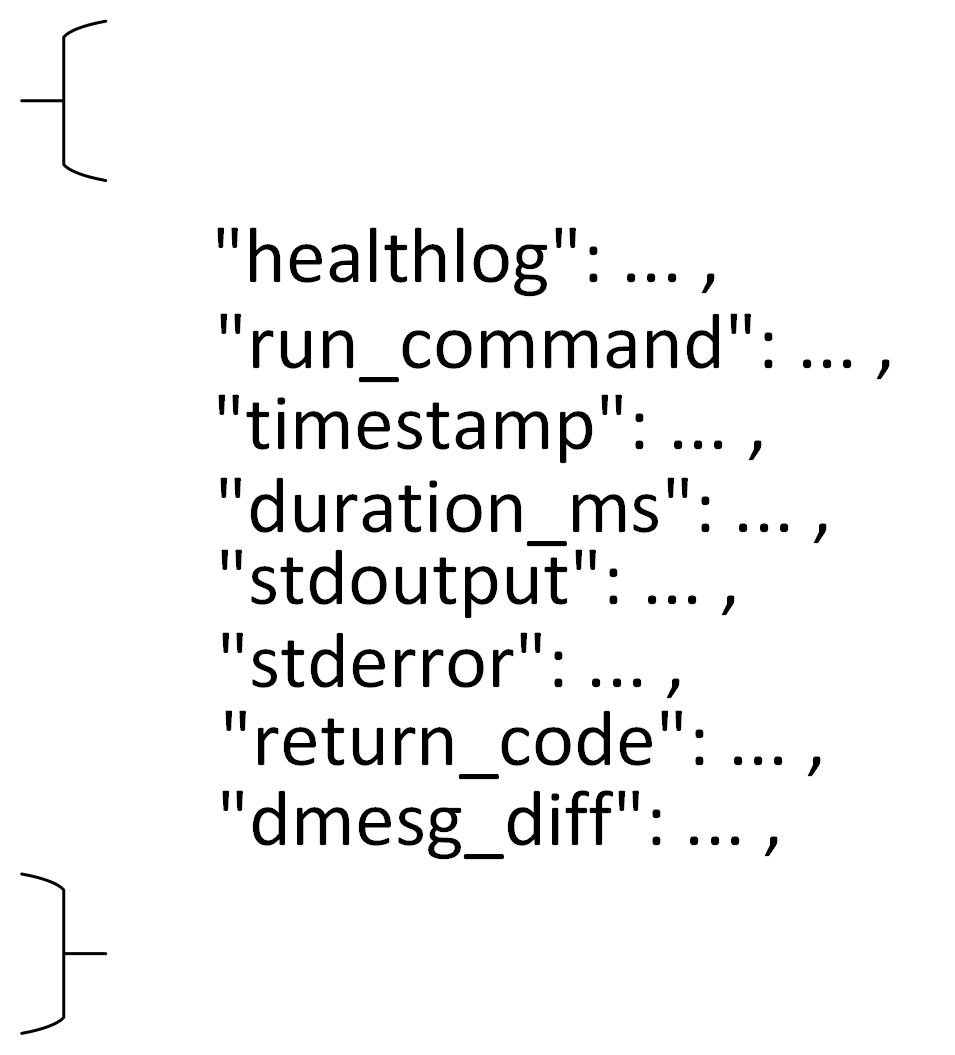
\includegraphics[width=\textwidth, height=7cm,keepaspectratio]{images/result_message_dut.png}
\centering
\caption{DUT's result message}
\label{fig:result_message_dut}
\end{figure}
\newpage